In this section only the relative position will be of interest therefore we introduce the reduced p.d.f,
\begin{equation*}
    P_\text{nst}(\textbf{r})
    =\int_0^\infty P_\text{nst}(\textbf{r},a) da,
\end{equation*}
which is the nearest pair probability integrated on all age of interaction. 
Also, the following graphs will be displays assuming an axis symmetry along the vertical axes. 
The horizontal plan will also be considered as a plan of symmetry even if the nearest pair probability density doesn't require that. 

\tb{it will be introduced above}


\paragraph*{Low inertial effects :}
We now present the reconstruction of the probability density function seen in the last section. 
We start by a meticulous analysis of $P_\text{nst}$ at low \textit{Galileo} number to investigate the effect of $\lambda$ and $\phi$ on the microstructure. 
As it will be seen in the next section the function $P_\text{nst}$ is not necessarily fore-after symmetric. 
Nevertheless, it turns out that for this specific case it was rather symmetric, therefore on the following histogram displayed  \label{fig:Pnst_low_Ga} and \label{fig:Pnst_high_Ga} we choose to show only the upper part of the distribution. 
\begin{figure}[h!]
    \centering
    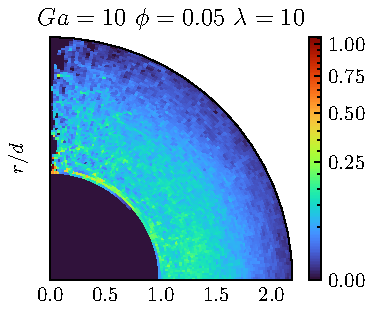
\includegraphics[height=0.2\textwidth]{image/HOMOGENEOUS_NEW/Dist/Pnst_l_10_Ga_10_PHI_0_05.pdf}
    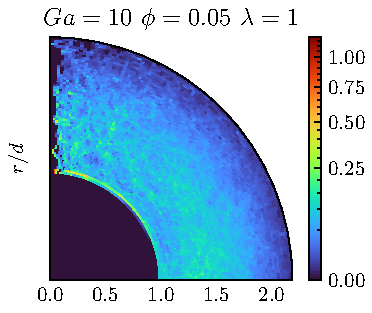
\includegraphics[height=0.2\textwidth]{image/HOMOGENEOUS_NEW/Dist/Pnst_l_1_Ga_10_PHI_0_05.pdf}
    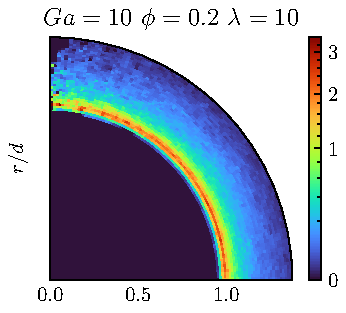
\includegraphics[height=0.2\textwidth]{image/HOMOGENEOUS_NEW/Dist/Pnst_l_10_Ga_10_PHI_0_2.pdf}
    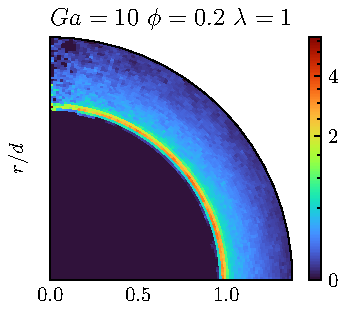
\includegraphics[height=0.2\textwidth]{image/HOMOGENEOUS_NEW/Dist/Pnst_l_1_Ga_10_PHI_0_2.pdf}
    \caption{Histogram of the probability density function $P_\text{nst}$ at low inertial effects $Ga = 10$.
    (left) Low volume fraction cases $\phi=0.05$ for $\lambda = 1,10$.
    (right) High volume fraction cases $\phi=0.1$ for $\lambda = 1,10$ }
    \label{fig:Pnst_low_Ga}
\end{figure}
At $Ga = 10$ we observe from \ref{fig:Pnst_low_Ga} that the probability of finding a nearest neighboring particle is even for all $\theta$. 
This is to say that $P_\text{nst}$ is isotropic for $Ga=10$.
If we compare the low versus high volume fraction case, we can remark that the PDF is more concentrated at $r = 2a$ for the latter case. 
This fact has been observed for solid particles \cite{guazzelli2011}, and we will see that it is even accentuated for higher inertial effects. 
Regarding the impact of the viscosity ratio, the PDF seem quite similar for two different value of $\lambda$. 
For instance, $\lambda$ seem to have no impact on the suspension microstructure. 

% \begin{itemize}
%     \item Regardless of $\phi$ and $\lambda$ the distribution is isotropic. 
%     \item The distribution seem to be more concentrated at $r=1$ for high $\phi$. 
%     \item Clearly the dilute simulation lack of statistical samples, however we can still see the tendency. 
% \end{itemize}